\documentclass{article}
\usepackage[UTF8]{ctex}
\usepackage{amsfonts}
\usepackage{amsmath}
\usepackage{float}
\usepackage{graphicx}
\usepackage{subcaption}
\usepackage{url}

\newcommand{\Bezier}{B\'ezier}%Bézier

\usepackage{color}

% paragraph
\setlength{\parindent}{0pt}
\setlength\parskip{\baselineskip}
\renewcommand{\baselinestretch}{1.2}

\begin{document}
	
	% 标题
	\title{《计算机辅助几何设计》作业}
	\author{ID号: 048  \qquad  姓名: 郑涛}  %递交作业时填上ID号和姓名
	\date{2024年11月22日}
	\maketitle
	1. Represent a unit sphere using a biquadratic rational B´ezier surface and draw it.
	
	2. Represent the ellipsoid $3x^2+2y^2+z^2=1$ using a bicubic rational B´ezier surface and draw
	it.
	
	The control points of one-eighth ellipsoid is:
	 $$p_{11}=(0,b,0),p_{12}=(a,b,0),p_{13}=(a,0,0)$$
	 $$p_{21}=(0,b,c),p_{22}=(a,b,c),p_{23}=(a,0,c)$$
	 $$p_{31}=(0,0,c),p_{32}=(0,0,c),p_{33}=(0,0,c)$$
	 weights of control points is:
	 \begin{equation*}
	 	W = \left(
	 	\begin{matrix}
	 		1&\frac{\sqrt{2}}{2}& 1\\
	 		1&\frac{\sqrt{2}}{2}& 1\\
	 		1&\frac{\sqrt{2}}{2}& 1
	 	\end{matrix}
	 	\right)
	 \end{equation*}
	
	\begin{equation*}
		x(u,v) = 
		\frac{\left(
		\begin{matrix}
			B_1^2(u)&B_2^2(u)&B_3^2(u)
		\end{matrix}
		\right)
		\left(
		\begin{matrix}
			W_{11}p_{11}&W_{12}p_{12}&W_{13}p_{13}\\
			W_{21}p_{21}&W_{22}p_{22}&W_{23}p_{23}\\
			W_{31}p_{31}&W_{32}p_{32}&W_{33}p_{33}
		\end{matrix}
		\right)
		\left(
		\begin{matrix}
			B_1^2(v)\\
			B_2^2(v)\\
			B_3^2(v)
		\end{matrix}
		\right)}
	{\left(
		\begin{matrix}
			B_1^2(u)&B_2^2(u)&B_3^2(u)
		\end{matrix}
		\right)
		W
		\left(
		\begin{matrix}
			B_1^2(v)\\
			B_2^2(v)\\
			B_3^2(v)
		\end{matrix}
		\right)}
	\end{equation*}
	use the dual weights:
	\begin{equation*}
		W = \left(
		\begin{matrix}
			1&-\frac{\sqrt{2}}{2}& 1\\
			1&-\frac{\sqrt{2}}{2}& 1\\
			1&-\frac{\sqrt{2}}{2}& 1
		\end{matrix}
		\right)
	\end{equation*}
	You can get the three-eighth ellsoid,then make half an ellipsoid center symmetrical.
	\begin{figure}[H]
		\centering
		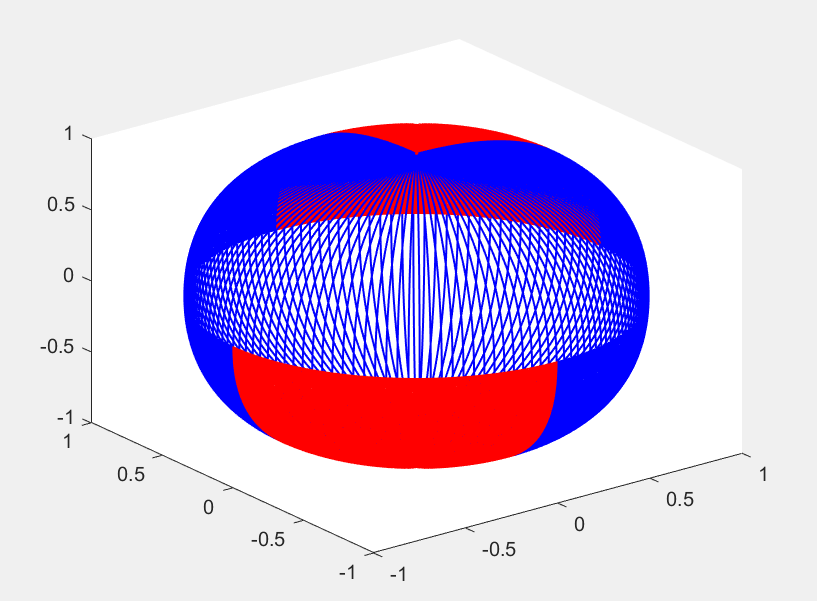
\includegraphics[scale=0.6]{1}
		\caption{$x^2+y^2+z^2=1$}
		\label{fig:1}
	\end{figure}
	
	
	\begin{figure}[H]
		\centering
		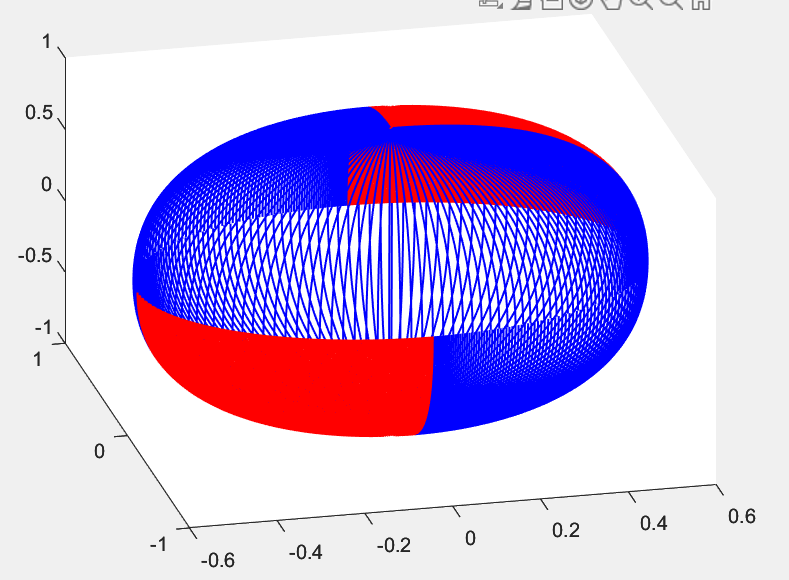
\includegraphics[scale=0.6]{2}
		\caption{$3x^2+2y^2+z^2=1$}
		\label{fig:2}
	\end{figure}

	3. A quadratic B´ezier triangle has vertex parameter coordinates a = (0, 0), b = (1, 0),
	c = (0.5, 1) and the following control points:
$$F(a,a)=\left(\begin{array}{c}	0\\0\\0 \end{array}\right),F(a,b)=\left(\begin{array}{c}	2\\2\\4 \end{array}\right),F(a,c)=\left(\begin{array}{c}	4\\-2\\6 \end{array}\right)$$
$$F(b,b)=\left(\begin{array}{c}	4\\4\\0 \end{array}\right),F(a,b)=\left(\begin{array}{c}	8\\0\\4 \end{array}\right),F(c,c)=\left(\begin{array}{c}	6\\-4\\4 \end{array}\right)$$
	Among the three parameters $p_1 = (0.25, 0.5), p_2 = (0.3, 0.75), p_3 = (0.5, 0.5)$, which parameter
	is outside the triangle? For the parameters inside the triangle, calculate the coordinates of
	the surface F(p, p) at these parameters using the de Casteljau algorithm.
	解:
	
	$p_2$ is out the triangle.
	
	\begin{equation*}
		\begin{aligned}
			F(p_1,p_1)=&F(\frac{a+c}{2},\frac{a+c}{2})\\
			=&\frac{F(a,a)}{4}+\frac{F(a,c)}{2}+\frac{F(c,c)}{4}\\
			=&\left(\begin{array}{c}	\frac{7}{2}\\-2\\4 \end{array}\right)
		\end{aligned}
	\end{equation*}
	\begin{equation*}
	\begin{aligned}
		F(p_3,p_3)=&F(\frac{a+b+2c}{4},\frac{a+b+2c}{4})\\
		=&\frac{F(a,a)}{16}+\frac{F(a,b)}{8}+\frac{F(b,b)}{16}+\frac{F(a,c)}{4}+\frac{F(c,c)}{4}+\frac{F(b,c)}{4}\\
		=&\left(\begin{array}{c}	5\\-1\\4 \end{array}\right)
	\end{aligned}
	\end{equation*}
\end{document}











